% !TeX root = ../main.tex
\section{Sensor Networks and Simplicial Complexes} % (fold)
\label{sec:complexes}

We consider the problem of determining coverage in a coordinate free sensor network.
That is, we would like to determine if an unknown domain is covered by a collection of sensors without their precise coordinates.
Let $\D$ denote our unknown domain and $P\subset\D$ be a collection of points, each representing a sensor in our network.
At the very least each sensor is capable of detecting nodes which are sufficiently ``close'' in the sense that, if we endow our domain with a metric $\dist:\D\times\D\to\R$ there is some radius of communication $\alpha > 0$ such that two nodes $p, q\in P$ such that $\dist(p, q) \leq\alpha$ are capable of communication.
Note that, although sensors can communicate within this distance they are not able to measure the distance itself.

We say that $D\subseteq\D$ is covered by $P$ at scale $\e > 0$ if every point $x\in D$ is within distance $\alpha$ at least one point in $P$.
Let $\ball_\e(p) = \{x\in\D\mid \dist(x, p)\}$ denote the \textbf{coverage region} of $p\in P$ at scale $\e$.
We will use the notation $P^\e$ to denote set of points in $\D$ within distance $\e$ of at least one point in $P$:
\[ P^\e = \bigcup_{p\in P}\ball_\e(p). \]
That is, $D\subseteq P^\e$ then the subset $D$ is \textbf{covered} by $P$ at scale $\e$.

With this limited capability we can construct an undirected graph $G=(V,E)$ with vertices $V=P$ and edges $E = \{\{p, q\}\subset P\mid \dist(p,q)\leq\alpha\}$.
In order to determine coverage we must at least assert that the coverage domain spanned by the points in $P$ does not contain any holes.
Assuming the coverage radius of our sensors is equal to their communication radius $alpha$ we may define a hole in coverage as a cycle that cannot be ``filled'' with triangles.
This leads us to a more natural construction known as a simplicial complex.

\begin{figure}[htbp]
\centering
    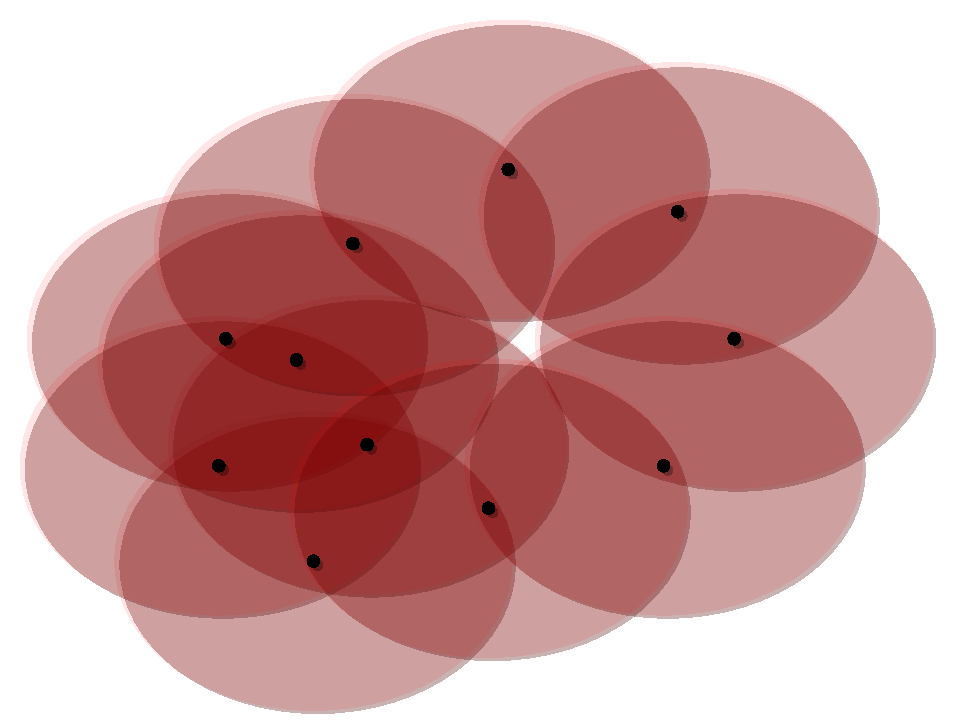
\includegraphics[scale=0.33]{figures/holes_cover.pdf}
    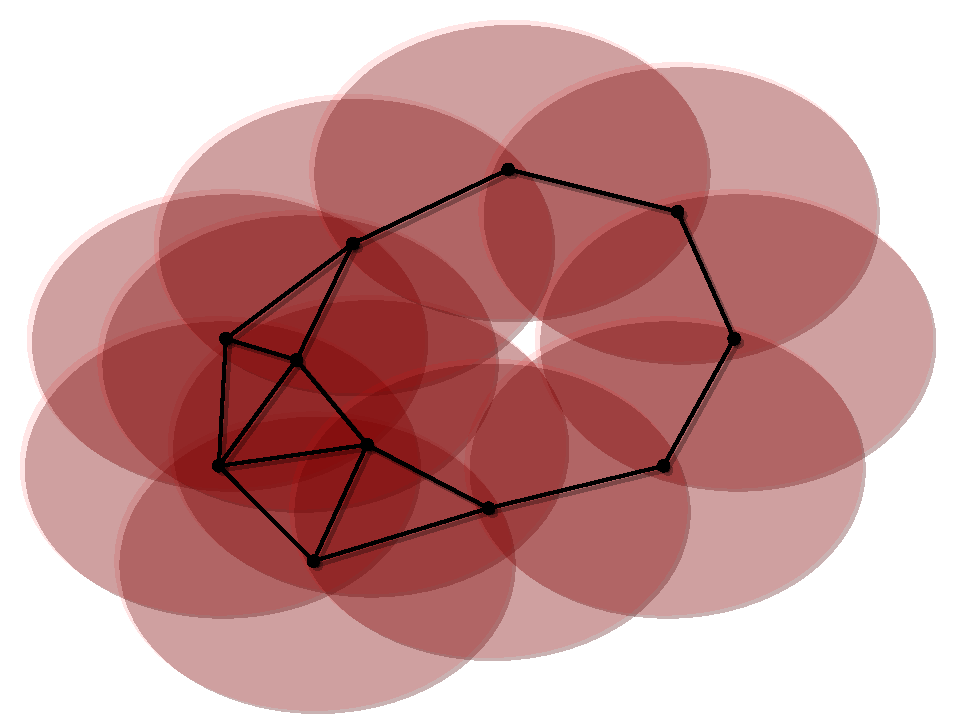
\includegraphics[scale=0.33]{figures/holes_edges.pdf}
    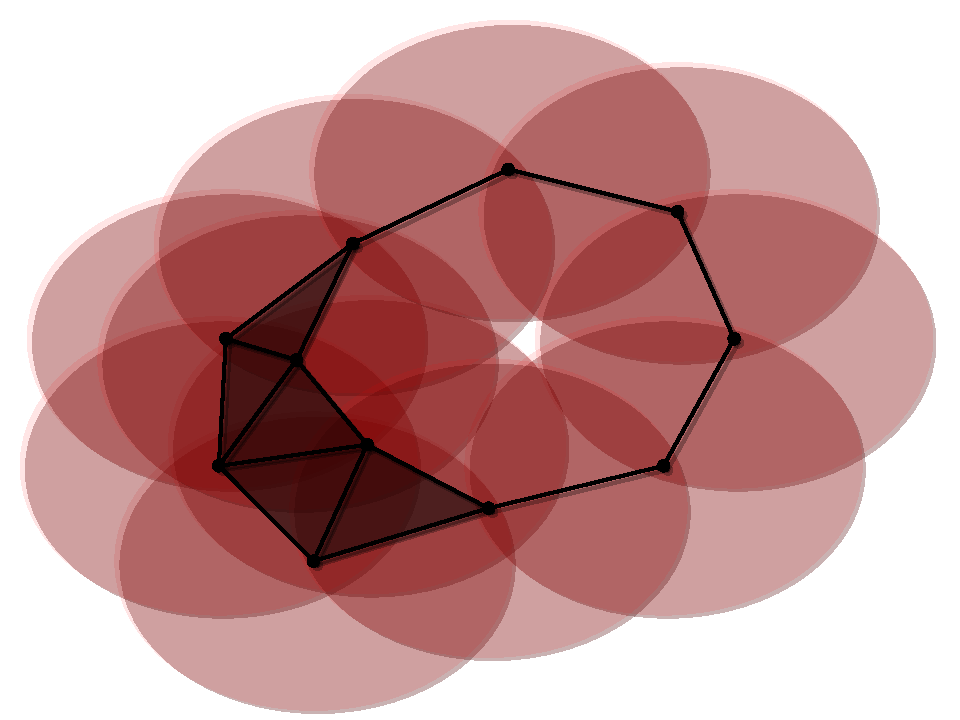
\includegraphics[scale=0.33]{figures/holes_complex.pdf}
     \caption{}
     \label{fig:holes}
 \end{figure}

\begin{definition}
    A \textbf{simplicial complex} $K$ is a collection of subsets, called \textbf{simplices}, of a vertex set $V$ such that for all $\sigma\in K$ and $\tau\subset\sigma$ it must follow that $\tau\in K$.
\end{definition}

Simplices may be thought of as a generalization of edges in a graph to higher dimensions.
The \textbf{dimension} of a simplex $\sigma\in K$ is defined as $\dim(\sigma) := |\sigma|-1$ where $|\cdot|$ denotes set cardinality.
The dimension of a simplicial complex $K$ is the maximum dimension of any simplex in $K$.
That is, a graph is a 1-dimensional simplicial complex in which vertices and edges are 0 and 1-dimensional simplices, respectively.

Recall, we have defined a hole in our graph as a cycle that cannot be filled with triangles.
If we instead construct a 2-dimensional simplicial complex in which a triangle, or 2-simplex, whenever 3 points are all within pairwise distance $\alpha$ a hole is simply a 1-cycle in the simplicial complex.
This particular simplicial complex is known as the Vietoris-Rips complex.
\begin{definition}
    The \textbf{(Vietoris-)Rips complex} is defined for a set $P$ at scale $\e > 0$ as
    \[ \rips^\e(P) = \left\{\sigma \subseteq P\mid \forall p,q\in\sigma,\ \dist(p, q)\leq\e\right\}. \]
\end{definition}
This construction generalizes to higher dimensions, allowing us to identify not only holes in planar graphs, ``holes'' in any dimension $k$ as $(k-1)$-cycles in high dimensional simplicial complexes.

\begin{figure}[htbp]
\centering
    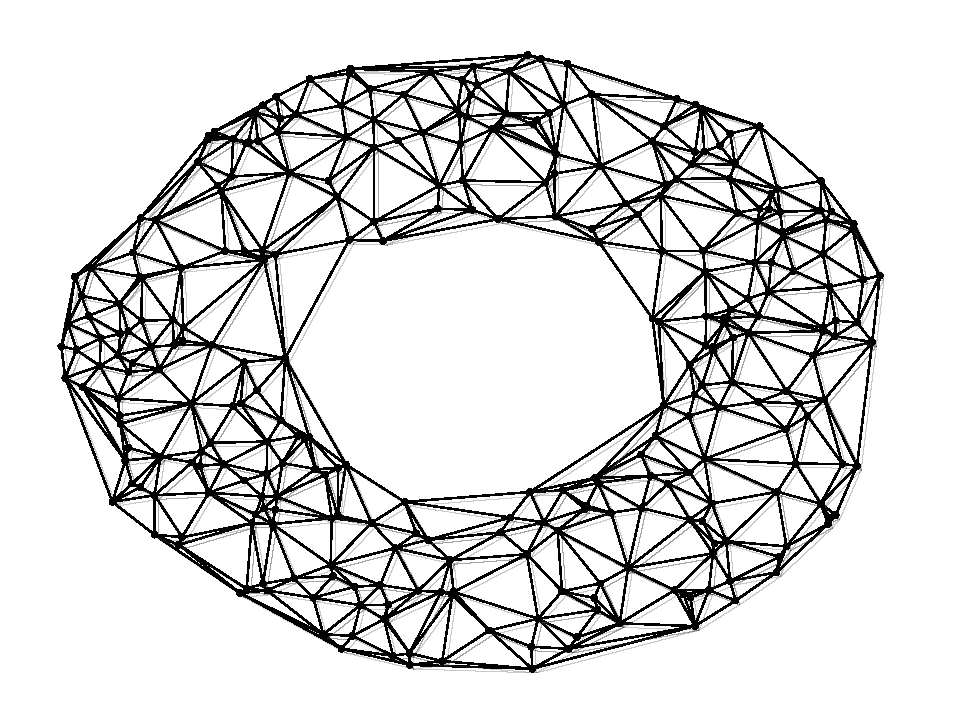
\includegraphics[scale=0.5]{figures/boundary_graph.pdf}
    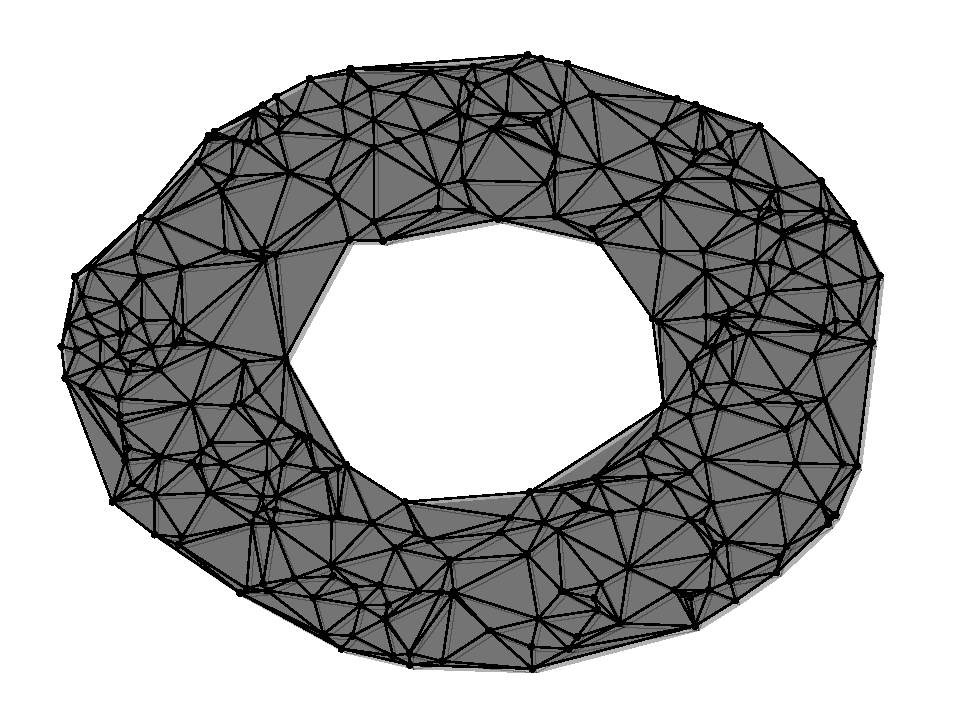
\includegraphics[scale=0.5]{figures/boundary_complex.pdf}
    % 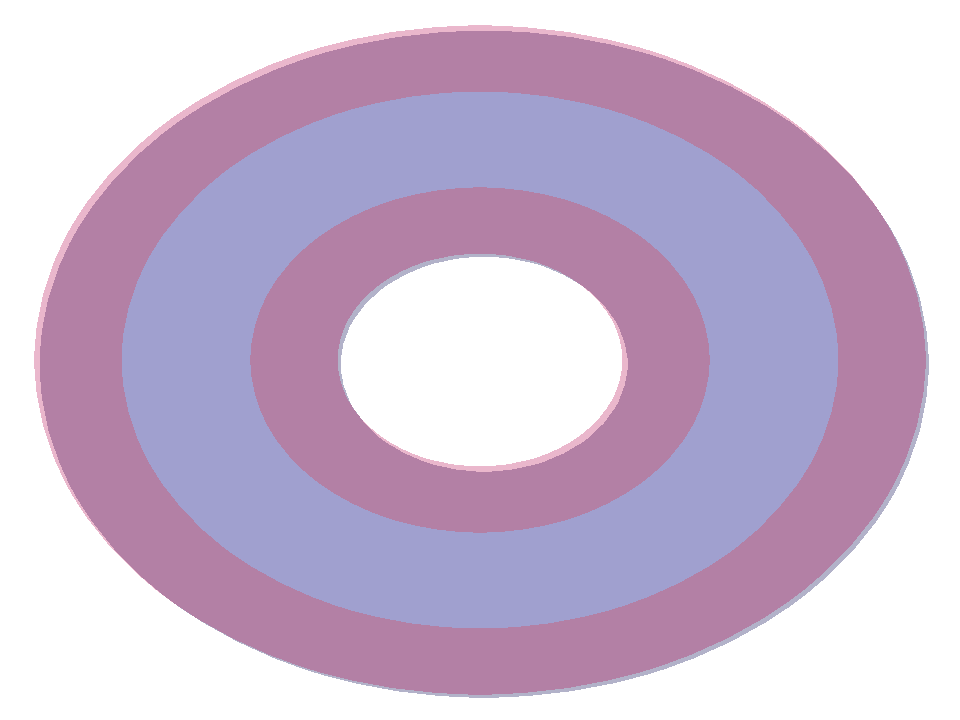
\includegraphics[scale=0.24]{figures/boundary_domain.pdf}
     \caption{}
     \label{fig:boundary1}
 \end{figure}

Once we have constructed a Rips complex $K = \rips^\alpha(P)$ we may identify gaps in coverage as ``unfilled'' cycles in the dimension of our domain.
However, even if we know there are no gaps in coverage how can we assert that our network sufficiently samples the domain?
Moreover, if there are gaps in coverage, are they due to insufficient sampling or a gap in the domain itself?
Both of these issues may be reconciled by allowing our sensors to detect the \textbf{boundary} $\B\subset\D$ of the domain.
Let $Q = \{p\in P\mid \min_{x\in\B}\dist(x, p)\}$ be the set of boundary nodes in $P$ and let $K\mid_Q = \rips^\alpha(Q)$ be the subcomplex of $K$ restricted to nodes in $Q$.
Now, way may say that a subset $D\subset\D$ is covered by our network at scale $\alpha$ if there are no holes in our network and no path from a simplex in $K$ to a point in $\D\setminus D$ without crossing a simplex in $K\mid_Q$.

\begin{figure}[htbp]
\centering
    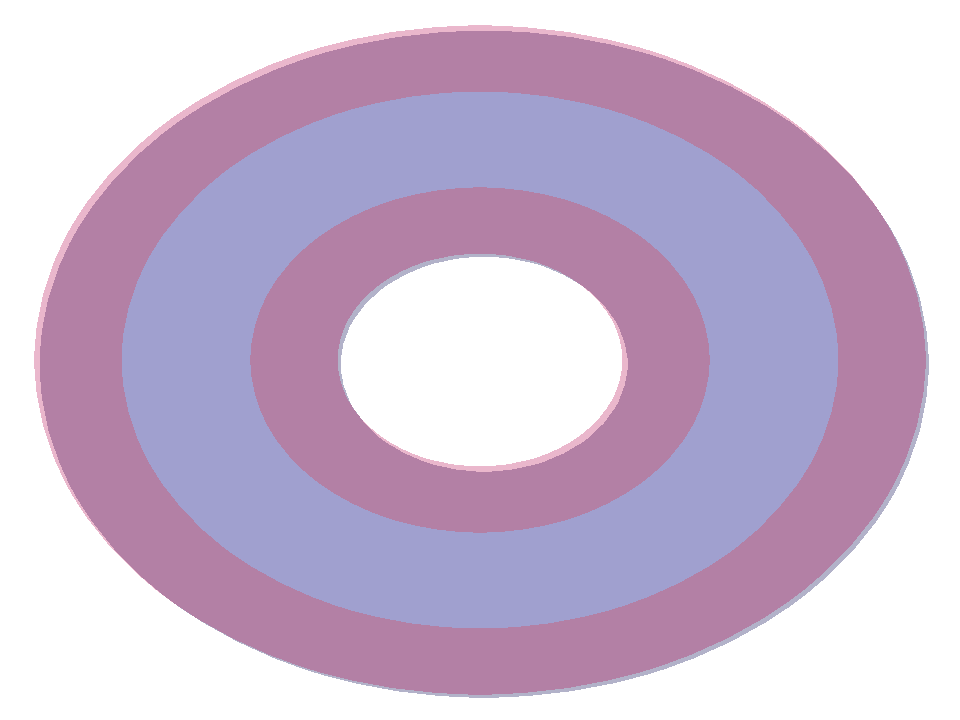
\includegraphics[scale=0.5]{figures/boundary_domain.pdf}
    % 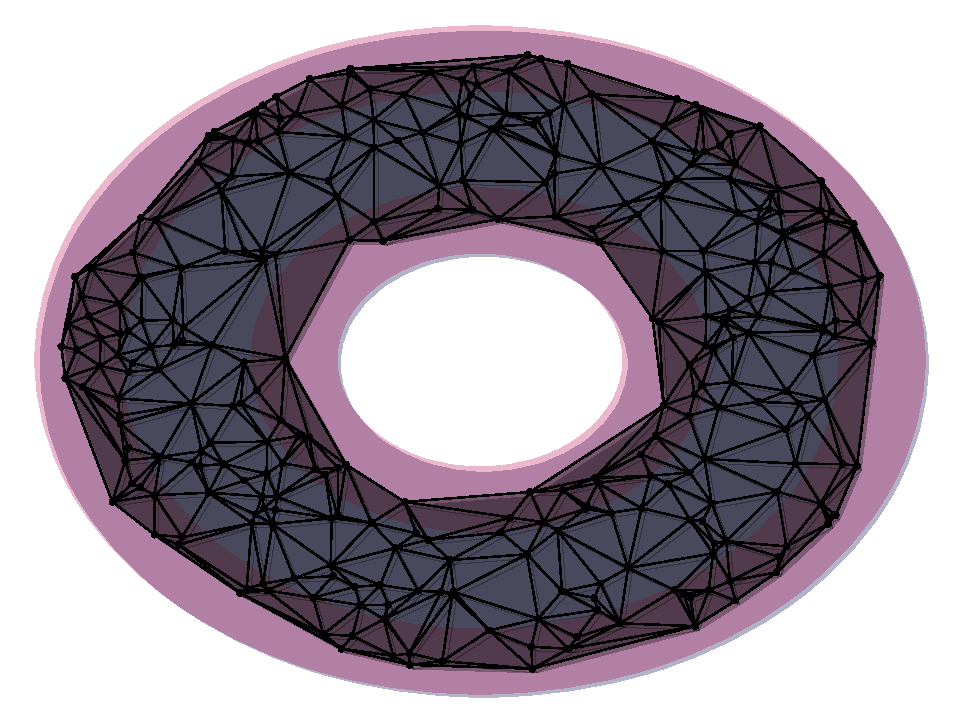
\includegraphics[scale=0.5]{figures/boundary_complex_domain.pdf}
    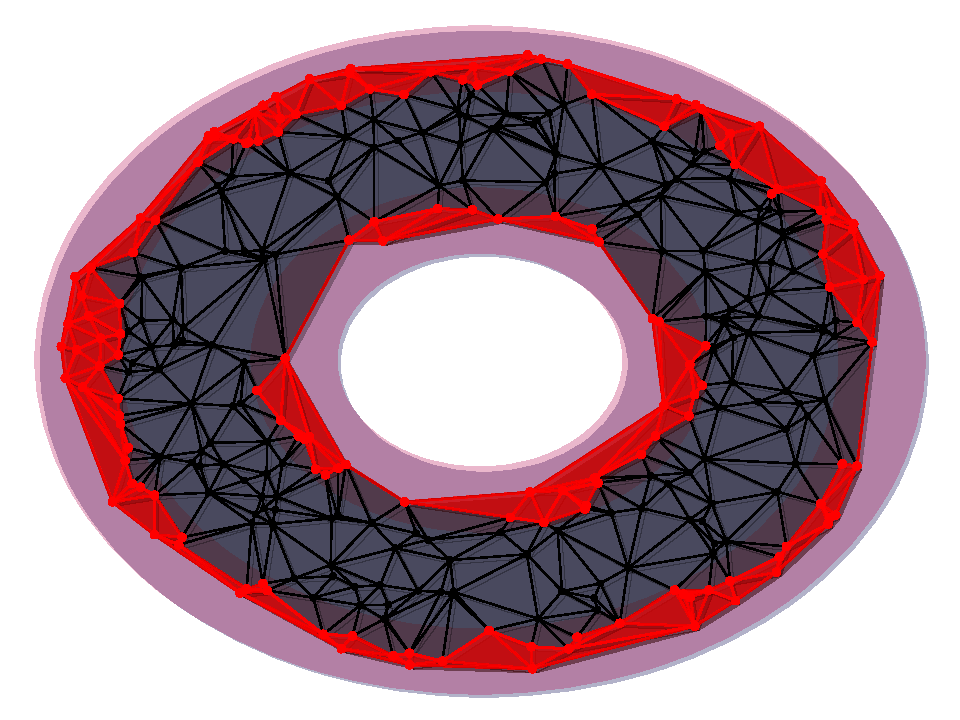
\includegraphics[scale=0.5]{figures/boundary_complex_domain_fence.pdf}
    % 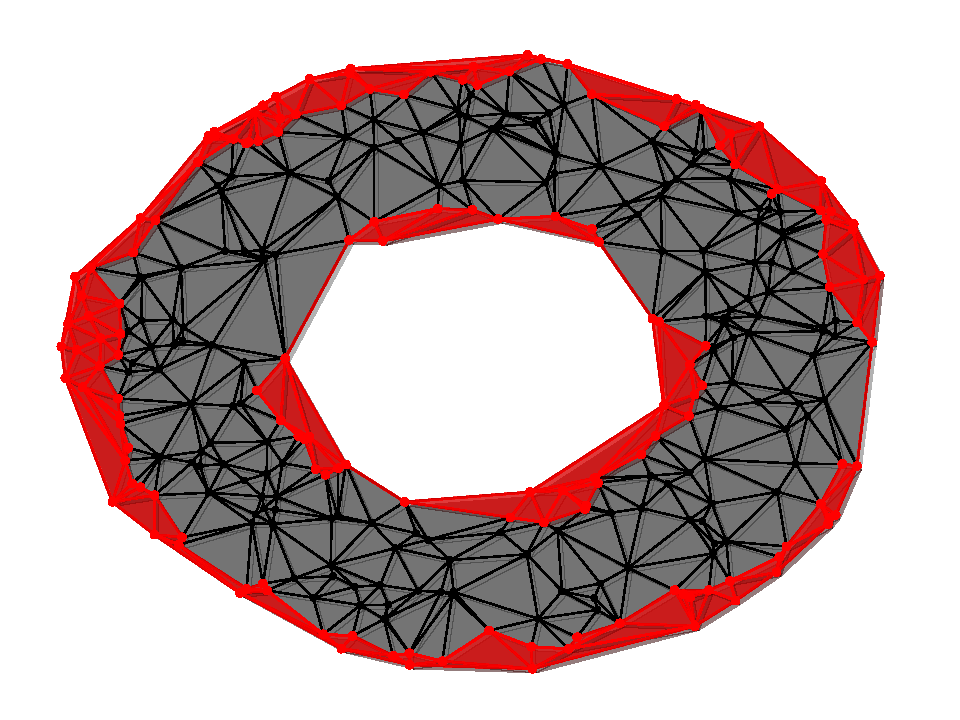
\includegraphics[scale=0.24]{figures/boundary_complex_fence.pdf}
     \caption{}
     \label{fig:boundary2}
 \end{figure}

Note that the communication radius is far from a tight bound on the coverage radius.
In section 5 we will detail precisely how to verify these conditions with a suitable coverage radius.

% section complexes (end)
